\section{Experiment}
To confirm that NaaA works widely with machine learning tasks, we confirm our method of supervised
learning tasks as well as reinforcement learning tasks. As supervised learning tasks, we use
typical machine learning tasks such as image classification using MNIST, CIFAR-10, and SVHN.

As reinforcement tasks, we confirm single- and multi-agent environment. The single-agent environment
is from OpenAI Gym. We confirm the result using a simple reinforcement task: CartPole. In
multi-agent, we use ViZDoom, a 3D environment for reinforcement learning.

\subsection{Classification}
\subsubsection{Setup}
%This experiment verified the performance of two tasks: classification and single-agent reinforcement learning.
For classification, three types of datasets were used: MNIST, CIFAR-10, and STL-10. 
The given task was to predict the label of each image, and each dataset had a class number of 10.
The first dataset, MNIST, was a collection of black and white images of handwritten digits sized 28�~28. The training and test sets contained 60,000 and 10,000 example images, respectively. 
The CIFAR-10 dataset images were colored and sized 32�~32, and the assigned task was to predict what was shown in each picture. This dataset contained 6,000 images per class (5,000 for training and 1,000 for testing).
The STL-10 dataset was used for image recognition, and had 1,300 images for each class (500 training, 800 testing). Each image was sized 96�~96; however, for the experiment, the images were resized to 48�~48 because the greater resolution of this dataset (relative to the above datasets) required far more computing time and resources.

\subsubsection{Model}
Two models were compared in this experiment: DropConnect and Adaptive DropConnect (the model proposed in this paper). The baseline model was composed of two convolutional layers and two fully connected layers whose outputs are dropped out (we set the possibility as 0.5). The labels of input data were predicted using log-softmaxed values from the last fully connected layer. In the DropConnect and Adaptive DropConnect models, the first fully connected layer was replaced by a DropConnected and Adaptive DropConnected layer, respectively. It should be noted that the DropConnect model corresponded to the proposed method when $\varepsilon$ = 1.0, meaning agents did not perform their auctions but instead randomly masked their weights.

\subsubsection{Results}
The models were trained over ten epochs using the MNIST datasets, and were then evaluated using the test data. The CIFAR-10 and STL-10 epoch numbers were 20 and 40, respectively. Experiments were repeated 20 times for each condition, and the averages and standard deviations of error rates were  calculated. Results are shown in Table \ref{tbl:cls}. As expected, the Adaptive DropConnect model performed with a lower classification error rate than either the baseline or DropConnect models regardless of the given experimental datasets.


\begin{table}[h]
	\caption{ Experimental result for image classification tasks and single-agent RL }\label{tbl:cls}. 
\centering
\begin{tabular}{l|ccc|c}
\hline
		& MNIST & CIFAR-10 & STL-10 & CartPole \\
\hline
		DropConnect \citep{wan2013regularization}	&	1.72 $\pm$ 0.160	&	43.14 $\pm$ 1.335	&	50.92 $\pm$ 1.322 & 285 $\pm$ 21.5 \\
		Adaptive DropConnect	&	\textbf{1.36} $\pm$ 0.132	&	\textbf{39.84} $\pm$ 1.035	&	\textbf{42.17} $\pm$ 2.329 & \textbf{347} $\pm$ 29.4 \\
\hline
\end{tabular}
\end{table}

\subsection{Single-agent RL}
Next, the single-agent reinforcement learning task was set as 
the CartPole task from OpenAI Gym \citep{openaigym} with visual inputs.
In this setting, the agent was required to balance a pole while moving a cart.
The images contained a large amount of non-useful information, making pixel pruning important.
The result in Table \ref{tbl:cls} demonstrates that our method improves the standard RL.

\subsection{Multi-agent RL}
The proposed reward distribution method was confirmed to work as expected by a validation experiment using the multi-agent setting in ViZDoom \citep{kempka2016vizdoom}, 
an emulator of Doom containing a map editor where additional agents complement the main player.
A main player in the ViZDoom environment aims to seek the enemy in the map and then defeat the enemy.

\subsection{Setup}
A defend the center (DtC)-based scenario, provided by ViZDoom platform, was used for this experiment.
Two players, a main player and a cameraman, were placed in the DtC, where they started in the center of a circular field and then attacked enemies that came from the surrounding wall.
Although the main player could attack the enemy with bullets, 
the cameraman had no way to attack, only scouting for the enemy.
The action space for the main player was the combination of \{ attack, turn left, turn right \}, giving a total number of actions $2^3 = 8$.
The cameraman had two possible actions: \{ turn left, turn right \}.
Although the players could change direction, they could not move on the field.
Enemies died after receiving one attack (bullet) from the main player, and then player received a score of +1 for each successful attack.
The main player received 26 bullets by default at the beginning of each episode.
The main player died if they received attacks from the enemy to the extent that their health dropped to 0, and received a score of -1 for each death.
The cameraman did not die if attacked by an enemy.
Episodes terminated either when the maim player died or after 525 steps elapsed.

\subsection{Model}
Three models, described below, were compared: the proposed method and two comparison targets.

{\em Baseline}: DQN without communication. The main player learned standard DQN with the perspective that the player is viewing.
Because the cameraman did not learn, this player continued to move randomly.

{\em Comm}: DQN with communication, inspired by Commnet. The main player learns DQN with two perspectives: theirs and that of the cameraman.
The communication vector is learned with a feed-forward neural network.

{\em NaaA}: The proposed method. The main player learned DQN with two perspectives: theirs and that of the cameraman.
Transmissions of rewards and communications were performed using the proposed method.

\begin{figure*}[t]
\centering
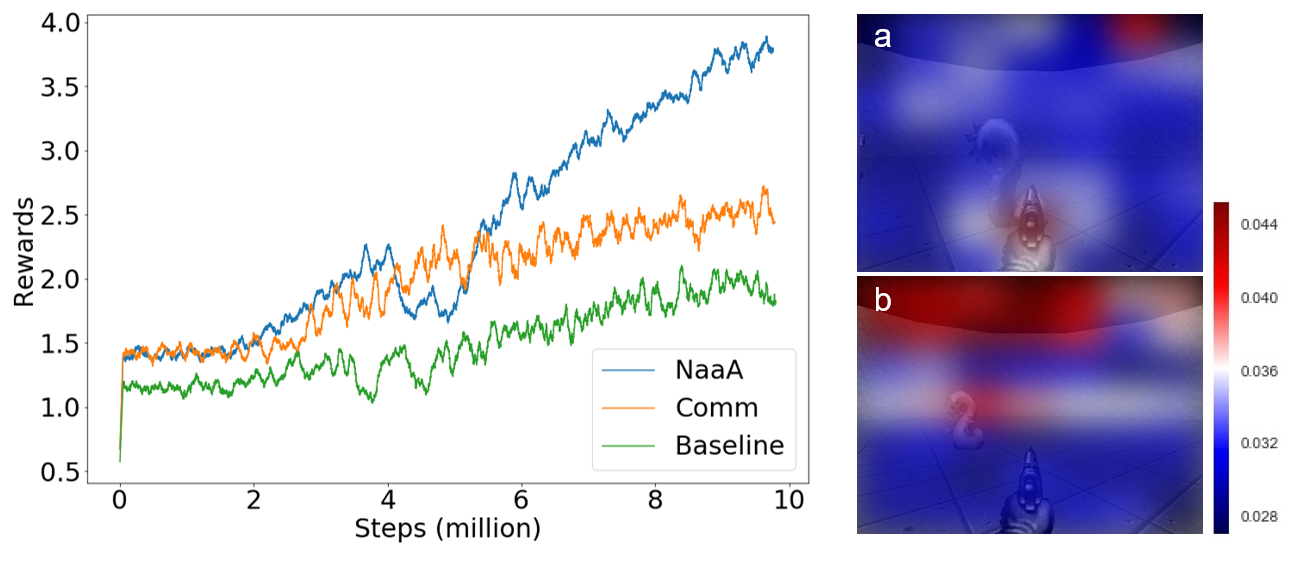
\includegraphics[width=\linewidth]{img/lc_vis.eps}
\caption{
	\textbf{Left:}
		Learning curve for ViZDoom multi-agent task. 
		The proposed NaaA--based method outperformed the other two methods (baseline and Comm DQNs).
	\textbf{Right:} 
		Visualizing reward from the main player to the cameramann shows us what is important information for the main player:
		(a) The pistol.
		(b) The point at which the enemy appeared and approached.
}
\label{fig:lc_vis}
\end{figure*}

\begin{figure*}[t]
\centering
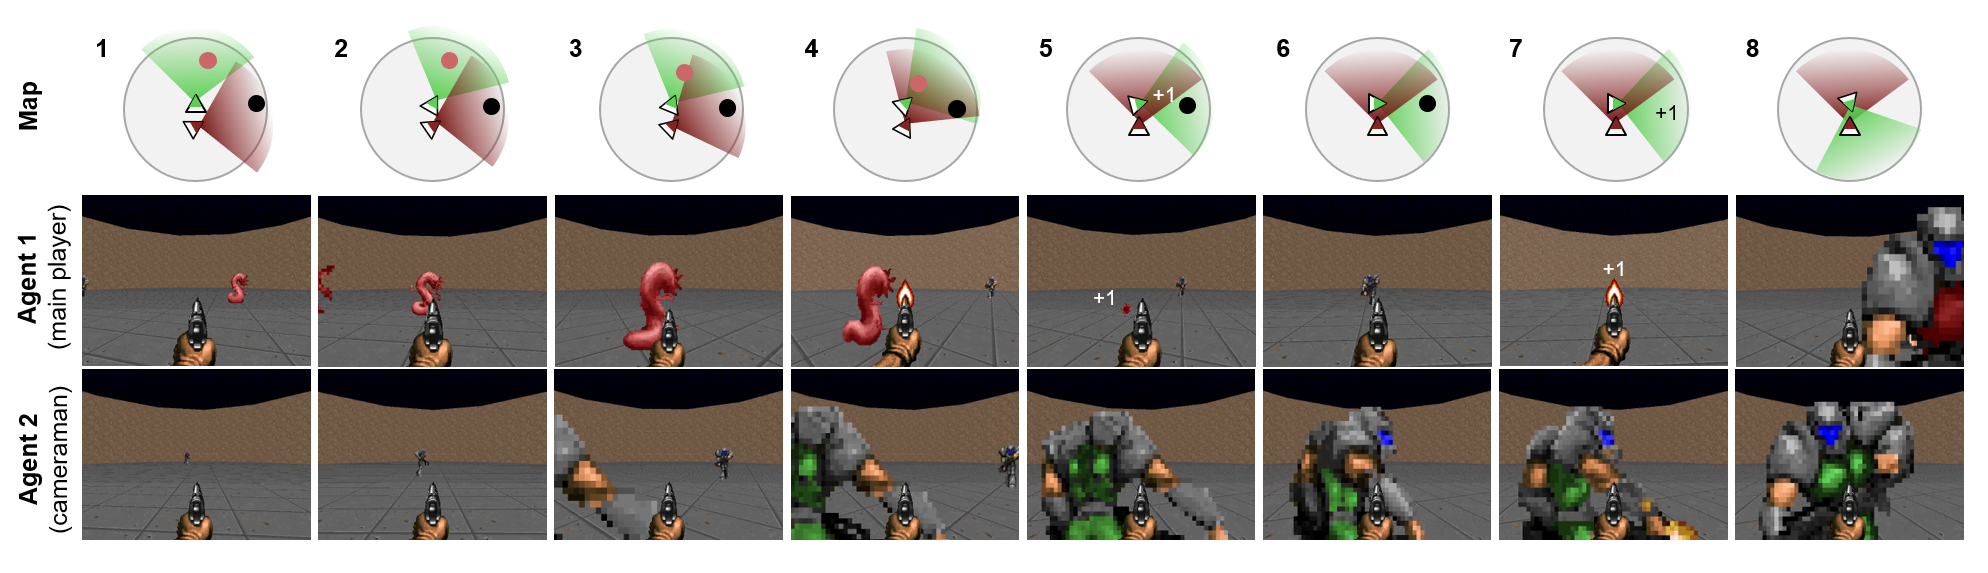
\includegraphics[width=\linewidth]{img/circleworld.eps}
\caption{
NaaA leads agents to enter a cooperative relationship.
First, the two agents face different directions,
and the cameraman sells their information to the main player (\textbf{1}).
The main player (information buyer) starts to turn right to find the enemy.
The cameraman (information seller) starts to turn left to seek new information by finding the blind area of the main player (\textbf{2} and \textbf{3}).
After turning, the main player attacks the first, having already identified enemy (\textbf{4} and \textbf{5}).
Once the main player finds the enemy, he attacks and obtains the reward (\textbf{6} and \textbf{7}).
Both agents then return to watching the dead area of the other until the next enemy appears (\textbf{8}).
}
\label{fig:circleworld}
\end{figure*}

\subsection{Results}
Training was performed over the course of 10 million steps.
Figure \ref{fig:lc_vis} Left demonstrates the proposed NaaA model outperformed the other two methods.
Improvement was achieved by Adaptive DropConnect.
It was confirmed that the cameraman observed the enemy through an episode, which could be interpreted as the cameraman reporting enemy positions.
In addition to seeing the enemy, the cameraman observed the area behind the main player several times.
This enabled the cameraman to observe enemy attacks while taking a better relative position.

To further interpret this result, 
a heatmap visualization of revenue earned by the agent is presented in Figure \ref{fig:lc_vis} Right.
The background picture is a screen from Doom, recorded at the moment when the CNN filter was most activated.
%The center corresponds to a position with the enemy appearing far away.
%The top corresponds to a position with the enemy coming closer.
%(b) shows that the agent sees the pistol.
Figure \ref{fig:circleworld} shows an example of learnt sequence of actions by our method.


%To confirm that NaaA works widely with machine learning tasks,
%we confirm our method of supervised learning tasks as well as reinforcement learning tasks.
%As supervised learning tasks, we use typical machine learning tasks such as image classification
%using MNIST, CIFAR-10, and SVHN.

%As reinforcement tasks, we confirm single- and multi-agent environment.
%The single-agent environment is from OpenAI gym.
%We confirm the result using a simple reinforcement task: CartPole.
%In multi-agent, we use ViZDoom, a 3D environment for reinforcement learning.

%The additional feature of NaaA is credit assignment for reward distribution, 
%meaning that if the neural network is divided into multiple agents, it works by playing the auction game.

